\documentclass{beamer}

\mode<presentation>
{
 \usetheme{Boadilla}
 \setbeamercovered{transparent}}

\usepackage[english]{babel}
\usepackage{times}

\usepackage{xcolor}
\usepackage{colortbl}
%\usepackage{subfigure}

%% for tables
\newcommand{\mc}{\multicolumn}
\newcommand{\lab}[1]{\multicolumn{1}{c}{#1}}
\newcommand{\ind}[1]{{\fboxsep1pt\raisebox{-.5ex}{\fbox{{\tiny #1}}}}}
\newcommand{\IND}[1]{{\fboxsep1pt\raisebox{0ex}{\fbox{{\small #1}}}}}
\newcommand\production[2]{\ensuremath{\langle\mbox{#1}, \mbox{#2}\rangle}}

%% markup
\newcommand{\buffer}[1]{{\color{blue}\textbf{#1}}}
\newcommand{\pred}[1]{\code{#1}}

%% colors
\newcommand{\textred}[1]{\alert{#1}}
\newcommand{\textblue}[1]{\buffer{#1}}
\definecolor{tablecolor}{cmyk}{0,0.3,0.3,0}
\newcommand{\keytab}[1]{\mc{1}{>{\columncolor{tablecolor}}d}{#1}}

% rules
\newcommand{\psr}[2]{#1 $\rightarrow \langle $ #2 $\rangle$}

\newenvironment{unpacked_itemize}{
\begin{itemize}
  \setlength{\itemsep}{10pt}
  \setlength{\parskip}{0pt}
  \setlength{\parsep}{0pt}
}{\end{itemize}}

\newcommand{\condon}{\hspace{0pt} | \hspace{1pt}}
\definecolor{darkblue}{rgb}{0,0,0.6}
\newcommand{\blueexample}[1]{\textcolor{darkblue}{\rm #1}}

%%%%%%%%%%%%%%%%%%%%%%%%%%%%%%%%%%%%%%%%%%%%%%%%%%%%%%%%%%%%%%%%%%%%%%

\newcommand{\ws}{\ensuremath{\vec{w}}}
\newcommand{\pu}{\ensuremath{P_0}}
\newcommand{\bx}{\mathbf{x}}
\newcommand{\bz}{\mathbf{z}}
\newcommand{\bd}{\mathbf{d}}
\newcommand{\by}{\mathbf{y}}
\newcommand\bleu{${B{\scriptstyle LEU}}$}


\title{Clustering of phrases and contexts}
\author{Trevor Cohn}
\date{\today}

\begin{document}

\begin{frame}[t]{Motivation}
%\vspace{1.0cm}
\begin{exampleblock}{Distributional Hypothesis}
\begin{quote}
\emph{Words that occur in the same contexts tend to have similar meanings}
\end{quote}
\hfill (Zellig Harris, 1954)
\end{exampleblock}

\vspace{3ex}

We will leverage this in a translation setting:
\begin{itemize}
    \item Use the contexts to \alert{cluster} translation units into groups
    \item Units in the same group expected to be semantically and syntactically similar
    \item Then use these cluster labels to guide translation
    \begin{itemize}
        \item lexical selection: translating ambiguous source word/s
        \item reordering: consistent syntactic patterns of reordering
    \end{itemize}
\end{itemize}
\end{frame}

\begin{frame}[t]{Monolingual Example}
Task: cluster words into their parts-of-speech. \\

\vspace{1ex}
Illustrate by starting with the word `deal' (noun or verb):

\only<1>{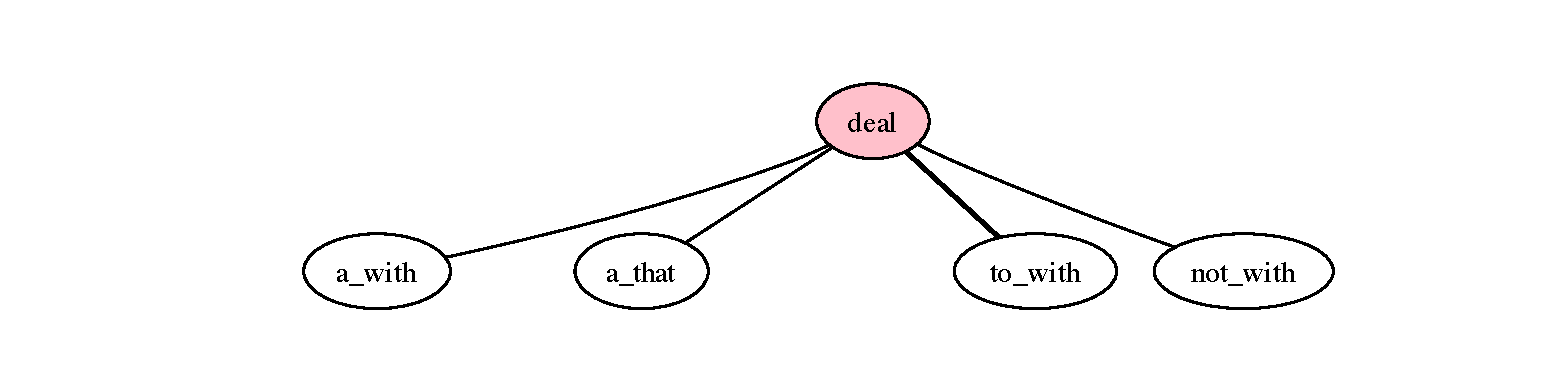
\includegraphics[width=\columnwidth]{deal_first.pdf} \\ Step 1: Find contexts for `deal'}
\only<2->{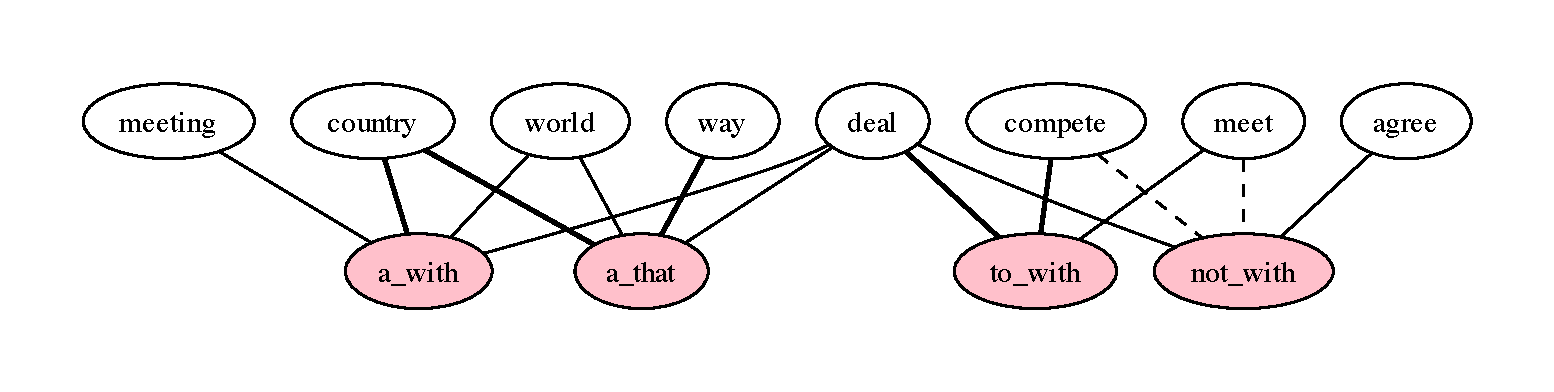
\includegraphics[width=\columnwidth]{deal.pdf} \\ Step 2: Find other words which occur in these contexts}
%\only<3>{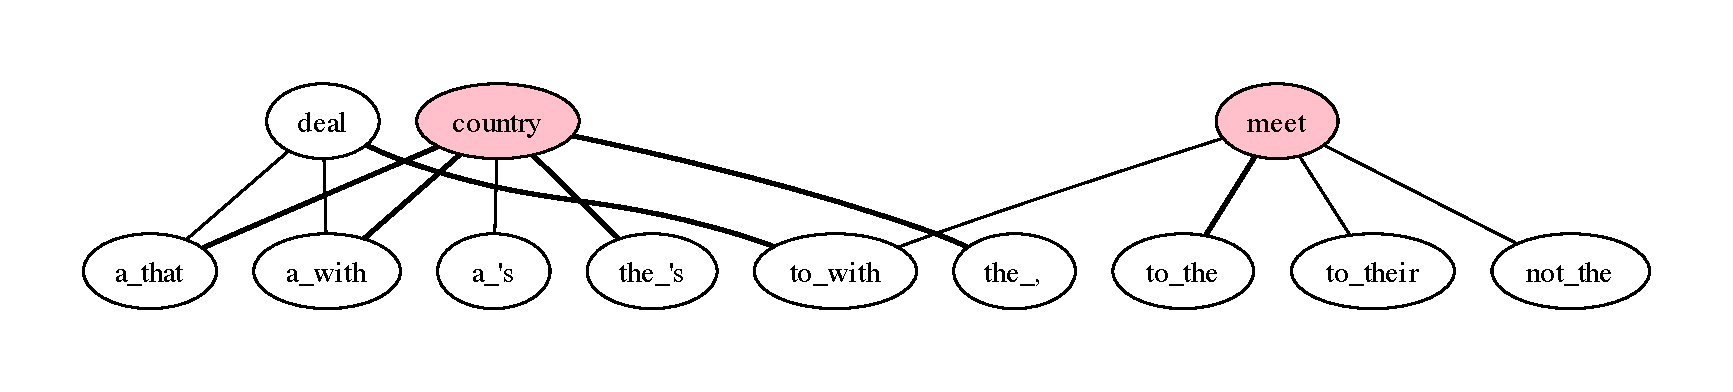
\includegraphics[width=\columnwidth]{deal_more.pdf} \\ \ldots continue to expand}

\only<3>{
\vspace{1ex}
Notice that the instances of deal can be split into two connected sub-graphs:
\begin{itemize}
    \item noun: the left two contexts ``a \ldots with'' and ``a \ldots that''
    \item verb: the right two contexts ``to \ldots with'' and ``not \ldots with''
    \item neighbouring words of these contexts share the same PoS
\end{itemize}
}

\end{frame}

\begin{frame}[t]{More Formally}

Construct a bipartite graph
\begin{itemize}
    \item Nodes on the top layer denote word types (bilingual phrase pairs)
    \item Nodes on the bottom layer denote context types (monlingual/bilingual words)
    \item Edges connect words and their contexts
\end{itemize}

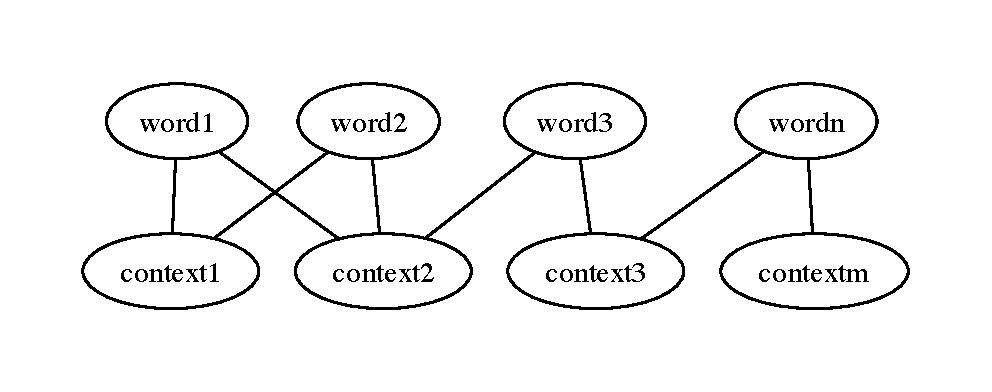
\includegraphics[width=\columnwidth]{bipartite.pdf}

\end{frame}

\begin{frame}[t]{Clustering}

Task is to cluster the graph into sub-graphs. Nodes in the sub-graphs should be
\begin{itemize}
\item strongly connected to one another
\item weakly connected to nodes outside the sub-graph
\item could formulate as either \emph{hard} or \emph{soft} clustering
\end{itemize}
Choose \alert{soft clustering} to allow for syntactic and semantic ambiguity

\centering
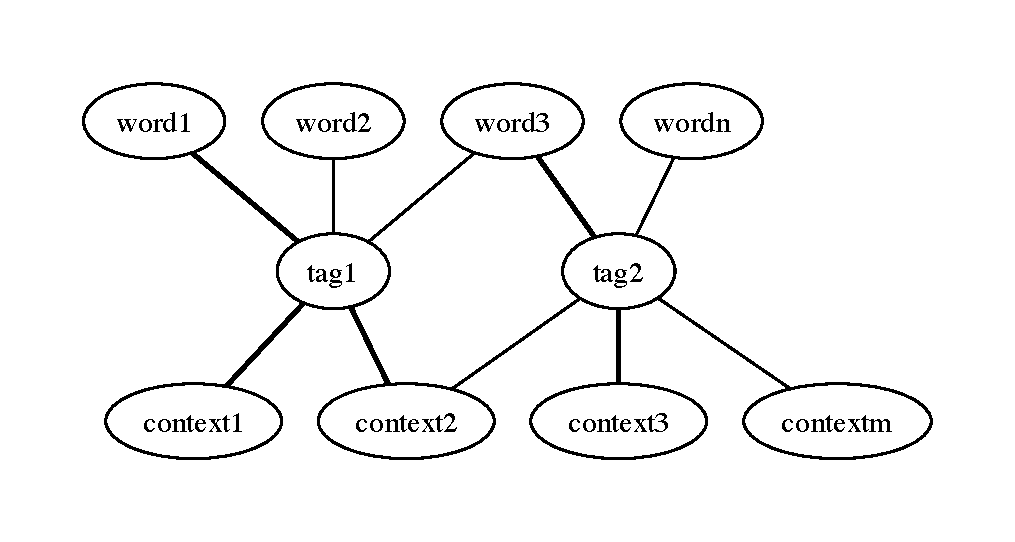
\includegraphics[width=0.7\columnwidth]{bipartite_lda.pdf}

\end{frame}

\begin{frame}[t]{Latent Dirichlet Allocation (LDA)}

LDA is a generative model which treats documents as bags of words
\begin{itemize}
    \item each word is assign a \alert{topic} (cluster tag)
    \item words are generated from a topic-specific multinomial
    \item topics are \alert{tied} across a document using a Dirichlet prior
    \item $\alpha < 1$ biases towards \alert{sparse} distributions, i.e., topic reuse
    \item inferred $\theta_d$ describes a document and $\phi_t$ describes a topic
\end{itemize}

\vspace{-3ex}
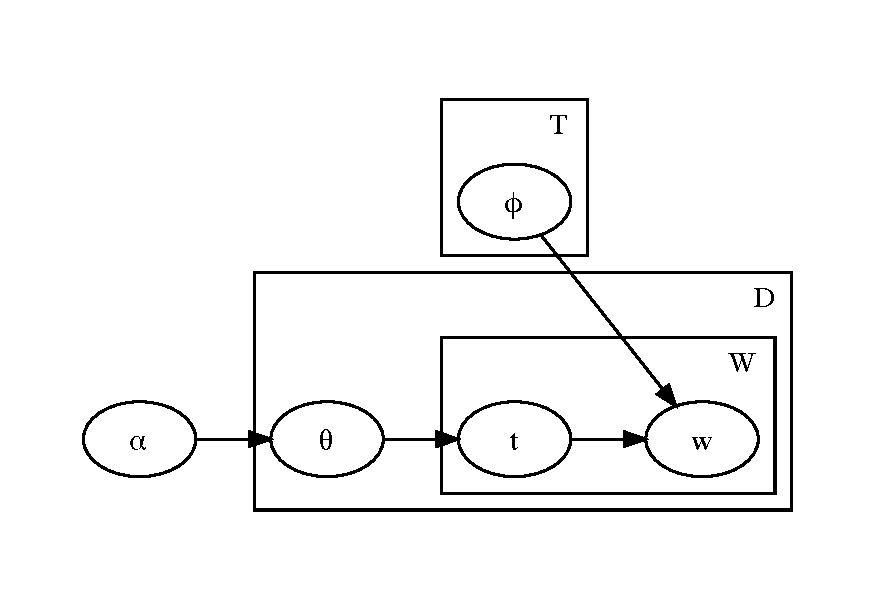
\includegraphics[scale=0.55]{lda.pdf}

\end{frame}

\begin{frame}[t]{LDA over Contexts}

Generative story:
\begin{itemize}
    \item for each word type $w$
    \item for each of the $L$ contexts
    \item first we draw a topic $t$, then generate the context $\vec{c}$ given the topic
    \item the Dirichlet prior ties the topics for each $w$
    \item we're primarily interested in the learnt $\theta$ values
\end{itemize}

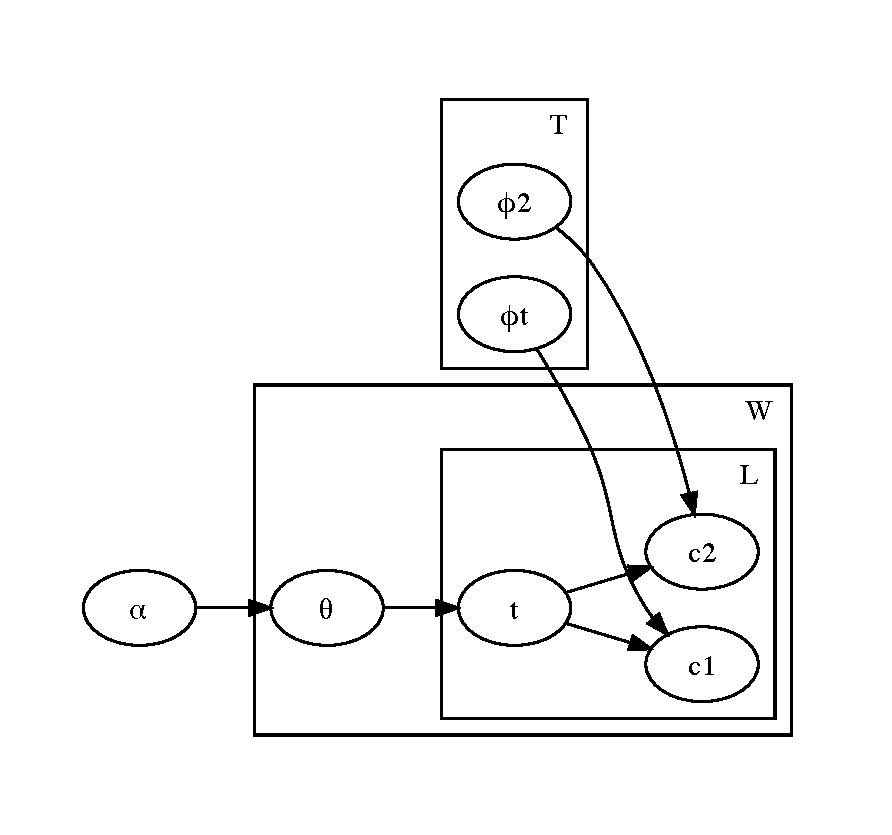
\includegraphics[scale=0.4]{context_lda.pdf}

\end{frame}

\end{document}
